\chapter{Conclusion}
\label{sec:conclusion}

This report has examined dark patterns not only as interface elements that may be present in an application, but also as exposure patterns that may vary across profile-conditioned interaction trajectories. This distinction matters because a user does not encounter an entire application at once. A user encounters a sequence of screens shaped by actions, searches, recommendations, prompts, and decision points. Profile-aware auditing therefore asks a more specific accountability question than static inspection: who encounters which forms of dark pattern exposure, how often, and under what behavioral conditions.

The proposed framework measures this problem through controlled profiles, repeated trajectories, and screenshot-level DPS annotation. Each profile is defined by interest and behavior distributions rather than demographic identity. Each observed screen is converted into a DPS vector covering Interface Interference, Friction, Pressure, Contextual Deception, Sneaking, Nagging, and Forced Action. Aggregating these vectors gives profile-conditioned exposure \(E(D \mid A)\), while pairwise comparisons provide differential exposure between profiles. In this design, dark pattern exposure is treated as a measurable distribution over interaction states, not as a single binary property of an app.

The empirical audit applied the framework to 16 apps, 3 profiles, and 30 steps for each app-profile pair, yielding 1,440 records and 10,080 DPS labels. The results suggest that exposure is unevenly distributed across controlled profiles. High-payment shopping and bargain-hunter trajectories more often encounter Pressure and Interface Interference, consistent with their movement toward checkout, membership, coupon, and promotion-heavy states. Low-payment browsing generally shows lower commercial-pressure exposure but still encounters Forced Action, Nagging, and access-control prompts. Category-level results further suggest that commercial, service, and engagement-oriented apps concentrate different DPS dimensions in different parts of the interaction path.

\begin{figure}[htbp]
    \centering
    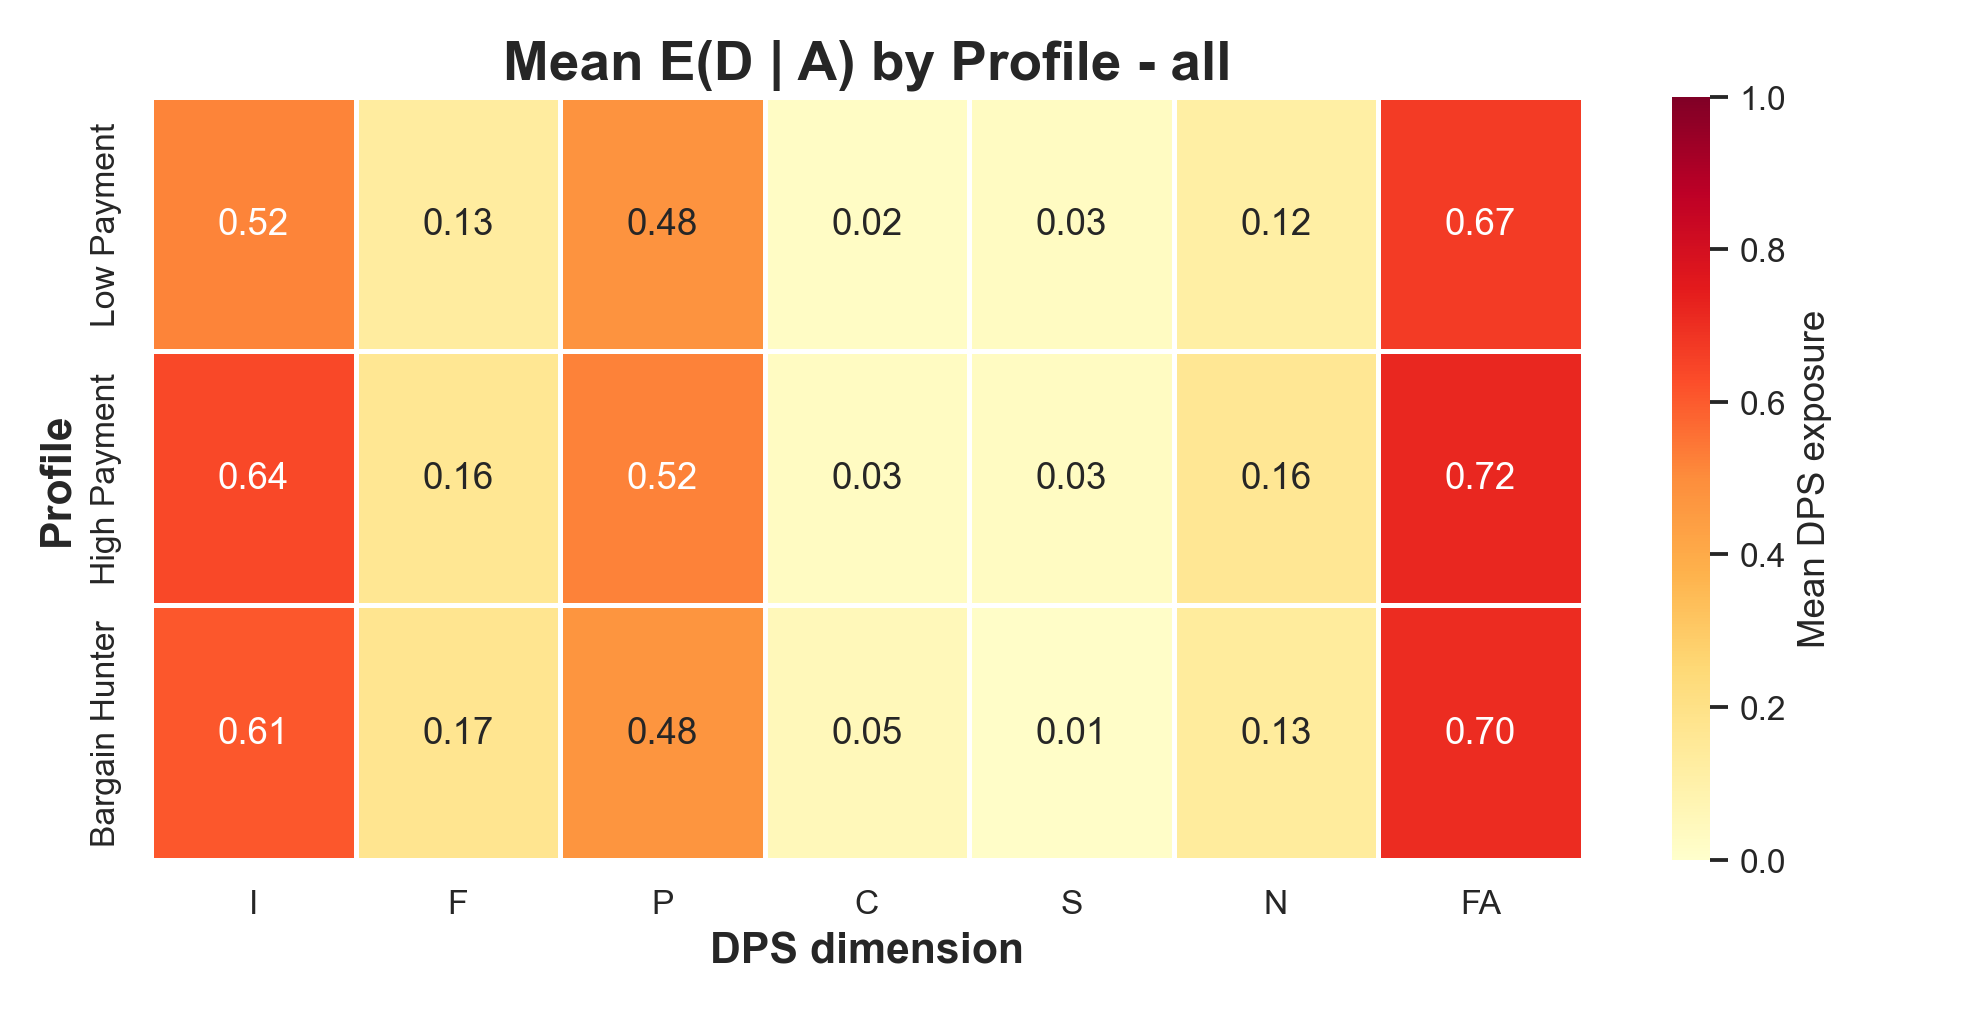
\includegraphics[width=0.95\linewidth]{figures/statistics/heatmap_mean_exposure_all.png}
    \caption{Summary heatmap of mean DPS exposure across all audited applications and controlled profiles.}
    \label{fig:conclusion-summary-heatmap}
\end{figure}

These findings do not imply deliberate profile-based manipulation. The audit observes visible outputs under controlled conditions; it does not inspect internal ranking, personalization, promotion, or interface-generation mechanisms. Differential exposure may arise from personalization, from rule-based app flows, from ordinary navigation differences, or from the fact that different profiles enter different decision contexts. The appropriate claim is therefore observational: in this dataset, profile-conditioned trajectories are associated with different DPS distributions.

Future work should extend the framework in several directions. Automatic or semi-automatic DPS annotation could reduce manual labeling cost while preserving human review for ambiguous cases. LLM-agent exploration could generate more realistic goal-directed trajectories than fixed probabilistic action sampling. Dynamic user modeling could examine how exposure changes as profiles accumulate interaction history. Larger audits across more apps, regions, versions, and time windows would improve external validity, while stronger statistical models could separate direct profile-associated exposure from exposure mediated by action pathways. Taken together, these extensions would move profile-aware auditing from a course-scale empirical framework toward a more scalable method for studying profile-conditioned exposure and platform accountability.
